
\begin{wrapfigure}{r}{4.5in}
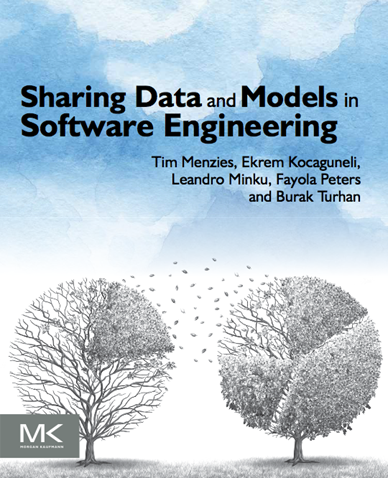
\includegraphics[width=1.45in]{fig/book1.png}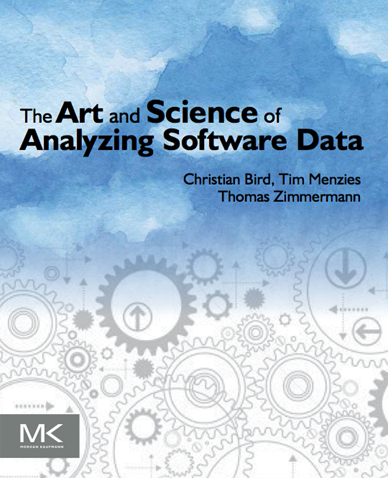
\includegraphics[width=1.45in]{fig/book2.png}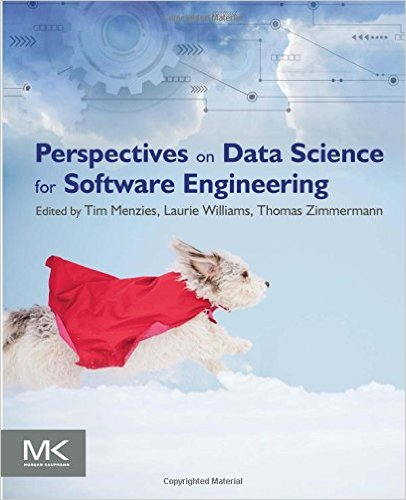
\includegraphics[width=1.45in]{fig/book3.jpg}
\caption{PI Menzies has co-written    three textbooks about 
empirical SE~\cite{menzies2014sharing,bird2015art,menzies2016perspectives}. But is any of that work relevant to
 computational science?}\label{fig:books}
\end{wrapfigure}


The previous section described ``what''  {\bf yields} we can collect from  different {\bf endeavors}.
This section describes ``how'' we will use those {\bf yields}, plus some other metrics,
to explore  Claims 1,2,3,4,5 from \tion{intro}.

In the following:
\bi
\item
  The metrics \#2,4,7,8,9 (described below)  address the claims listed in \tion{intro} while the
 other metrics address   specific requirements
of the CSSI solicitation.
\item
Most of the following metrics are qualitative in nature. The exception is Metric \#8
which will allow a rigorous statistical test of the value of {\IT}. For more on those tests,
see the discussion on {\bf Claim5} at the end of \tion{other}. \ei
\noindent
\subsection{Architecture}   {\IT} will be written in JAVA/Python and 
combine tools from several existing open source toolkits such as 
Scikit-Learn~\cite{scikit-learn}, jMETAL~\cite{durillo2011jmetal}, and Commit.Guru~\cite{commitguru}.
To that suite of software we will add tools recently developed in PI Menzies's lab including
the data processors of Agrawal etl'18~\cite{agrawal2017better}; 
the FLASH hyperparameter  optimizer~\cite{nair2017flash};
the FASTERAD active learner~\cite{Yu:2018,Yu2019}; as well as code
from several other prototoypes (all the code used to generate the    Figure~2 result;
the test prioritization methods tested in \fig{relative};  
the warning analyzer used in    \fig{warn};  
and the technical debt analysis tools used in \tbl{SATD},
\fig{warn}~\cite{xia19}). Further, as the research in our lab continues,
we foresee that other, newer, tools will also be added to {\IT}.





{\IT} will also contain data files holding all the features we extracted from \tbl{samples}. This is useful
since it will allow other researchers to quickly repeat/improve/refute our results without having
to first perform tedious web-scale data collection.

{\IT} will also contain the source core required to reproduce 
our proof-of-concept papers (discussed below). For example, if  a  paper
has research questions RQ1, RQ2, then our code will come with shell scripts
 RQ1.sh, RQ2.sh etc that store the code we executed to answer the research questions.


\subsection{Adaptability to New Technologies} Toolkits like Scikit-Learn and jMETAL
  are currently the international distribution method
for new data mining and optimization
algorithms. Hence, whenever Scikit-learn or jMETAL changes, {\IT} will be positioned to access
and use the  latest innovations  

\subsection{Adaptability to Changing Requirements}
As stated above, this proposal will use {\IT} to explore the four {\bf endeavors}
described above as well as  other tasks as time and opportunity permits and as requested by computational scientists.
We will maintain a roadmap document so that if (for pragmatic reasons)
we cannot currently explore a particular new requirement,
our users will know when they can expect that new functionality.


\subsection{Delivery and Outreach Mechanism}\label{tion:outreach}  {\IT} will
be licensed
open source and
stored in a public
 repository
 that anyone can download and run on their own machines. When executed, these tools
can automatically  work through on-line data from computational science projects.  


{\IT}
will be delivered using Github (i.e. using the
{\tt git clone} command)\footnote{If possible, we will also offer Docker files to distribute our system.
That said, the practicality
of that proposal has to be assessed further once we know the size of the shared data sections
in {\IT}.}. 

We anticipate  that {\IT} will need no proprietary licensed products. Hence  {\IT}
will cost \$0.


As to outreach,
 we would work with the organizers of the annual $SI^2$ PI meeting to arrange focus groups at that meeting
 (so we can have detailed  interaction with interested developers).
In-between the $SI^2$ PI meetings, we would also 
run tutorials on our tools (and related concepts in Empirical SE)
at the PEARC conference (one per year)
as well as webinars
for XSEDE  
and the Sciences Gateways series (whenever we have anything interesting to report).
Accordingly, we will log and report:
\bi
\item {\em METRIC0: Number of tutorials given on this material.}
\ei

\subsection{Timeline}
In the first few months of the project, in order to quickly obtain more initial results (which we can use to popularize this project
and raise its profile in the computational science community), we will apply {\IT} to extend the case study of Figure~2, using the rest of the projects in \tbl{samples}.
After that, for the first two years of this work we will spend six months on each
of the endeavors (a)(b)(c)(d) listed in \tion{ende}. 
For the third year, we will look over our tools to see what can be generalized, improved, simplified. This will lead to a code re-organization.
Apart from that, in all years:
\bi
\item
We will not have releases {\em per se} but a continuous integration
of development and code, ready to be used.
To that end, {\IT}
will be stored open source and on-line to be freely available during+after
this proposal. That is,  just as soon as our tools get useful, they will be
available to the general computational science community.
\item
We will use {\IT} to generate numerous proof-of-concept reports;
i.e. two to four research publications per year, ideally
at top-ranked values.
These proof-of-concept papers would be our reports on what happens when we applied 
empirical SE methods to computational science projects. 
\ei
Accordingly we will log and report:
\bi
\item {\em METRIC1: Number of written/published proof-of-concept papers.}
\ei
\subsection{Reproduciblility }
 As stated above,
all our proof-of-concept papers will come with on-line replication packages
with scripts labelled RQ1.sh, RQ2.sh etc that store the code we executed to answer the research questions
of those papers. 


\subsection{Testing and Documentation}
The proof-of-concept reports will be the
systems-level tests of {\IT}.
As to documentation, we   commit to  maintaining  the standard of documentation proposed
in the Code Carpentry  paper {\em Good Enough Practices for Scientific Computing}~\cite{Wilson16} which include an {\tt INSTALL.md} files describing downloading
an installation plus {\tt README.md} files describe example usages of the system.
As to other documentation, we will use a literate  programming style of documentation; i.e.
or Jupyter notebooks;  
 code and classes docs generated  from  code,
presented in a public  {\tt /docs} directory in
our repos.



\subsection{User Interactions} We would create a simple on-line registration Google
form  where interested developers can register their repository with us. Accordingly, we will log and report: 
\bi
\item {\em METRIC2: How many projects register themselves for our service.}
\ei
Our agents will then analyze the 
registered projects using our automatic agents,
posting   issue reports back to those repositories.
Accordingly, we will log and report: 
\bi
\item {\em METRIC3: Number of projects analyzed.}
\ei
We will  track if those issues
are ever acted on by  projects (and if none are, then that would indicate our tools are reporting
irrelevancies). Accordingly, we will log and report: 
\bi
\item {\em METRIC4: How computational scientists change their projects
in response to our recommendations.}
\ei
As to day-to-day support of teams using our tools,
some of  their time will be dedicated
to offering   support and advice to  those computational science teams.
Accordingly, we will log and report
\bi
\item {\em METRIC5: Number of help requests from how many projects (trying to run our tools on their code).}
\ei
Since our code will be on-line in a web-accessible repository, we will also be able
to gauge the community's interest in our work via the number of pull requests and issue
or
bug reports posted to our repository:
\bi
\item {\em METRIC6: Number of pull requests and issue or bug reports.}
\ei
\subsection{Security} 
We do not anticipate security issues for this project since we will using data that the projects are already placing on-line.

 
 
\subsection{Other Metrics}\label{tion:other}
The above Metrics \#2,4,5,6 (as well as some that follow)  measure
user involvement in this project. They also let us see to what extent
users accept our new tools.

The rest of this section discusses the metrics required
to explore  the
five claims of \tion{intro}.   

To  explore   {\bf Claim1 = relevance}, we must try
to interest   computational scientists in our methods.
For that task, we will use the above mentioned
Metrics \#2,4.    That is to say, we will use computational scientist to judge if what we are doing
is worthwhile.  Note that we all ready have some preliminary indications that we may do well
according to Metric \#2 (see the 11 letters collaboration attached to this proposal).

Given the wide ranging nature of this
proposal, it may not be true that all our future
work as simple as seen in the Figure~2 case study.
Therefore, to explore  {\bf Claim2 = operational} we must log and report:
\bi
\item {\em METRIC7: The human effort
 required to apply the SE {\bf instrument}.} 
\ei
Metric \#7 will record how hard for humans to  {\bf tune} and {\bf instrument} for computational
science. But are their any benefits justified with respect to  the cost of {\bf tuning}?
To make that assessment, in order to justify,
 \mbox{{\bf Claim3 = must adjust}}, we must log and report:
\bi
\item {\em METRIC8: compare the  performance 
scores {\bf yielded}
using standard empirical SE {\bf instruments}, before and after {\bf tuning}.}
\ei
Note that one unlikely, but very useful result,
would be that the {\bf yield} does not
increase after {\bf tuning}
standard empirical SE methods for computational
science projects. In that case, {\bf Claim3} would be refuted.
Having recorded that possibility, we note that this is very unlikely.
Firstly, the nature of computational science software is very different to the Google- and Facebook- and Microsoft- style of projects used to develop current empirical SE
methods. Secondly, the experience of Figure~2 is that significant adjustments are required
to standard empirical SE methods before they are effective for computational science.

To explore {\bf Claim4 = practical}
we must log and report the effort required to 
adjust SE methods to computational science; specifically:
\bi
\item {\em METRIC9: the CPU time or other platform  costs
required to complete tuning.}
\ei
This metric is subtly different to Metric \#7. In the prior metric, we checked
the difficulty for humans to wrangle together a working system. In this metric we 
measure the cost of the hardware systems (computer hardware,  cloud compute costs, CPU time).
This is an important point since some {\bf tuning}
{\bf strategies}
can be impractically slow~\cite{abs-1807-11112},
particularly if those {\bf strategies} need to be repeated
many times during a rapidly evolving software project.
Worse, if those {\bf strategies} themselves have
to be changed from project to project there we
would be unable to offer any guidelines on how to best
{\bf tune} the next project.

To explore  {\bf Claim5 = valuable}, we would reuse
{\em Metric8} and reflect on the 
  {\em size} of the {\bf yield} difference seen after
  applying empirical SE methods (with or without
  {\bf tuning}, depending on the results of {\bf Claim3}).
  \bi
  \item
  This test would use some statistical significance and
  effect size test (e.g. a 95\% bootstrap sample and Cliff's Delta).
  \ei
  Note that if,
  at the end of the day, empirical SE offers very
  little benefit for computational  science, then we would reject Claim5 and declare
  a negative result from this research.
  
  